\documentclass{beamer}
\usepackage[utf8]{inputenc}

\usetheme{Madrid}
\usecolortheme{default}
\usepackage{amsmath,amssymb,amsfonts,amsthm}
\usepackage{txfonts}
\usepackage{tkz-euclide}
\usepackage{listings}
\usepackage{adjustbox}
\usepackage{array}
\usepackage{tabularx}
\usepackage{gvv}
\usepackage{lmodern}
\usepackage{circuitikz}
\usepackage{tikz}
\usepackage{graphicx}
\usepackage{textcomp}
\usepackage{cancel}
\setbeamertemplate{page number in head/foot}[totalframenumber]

\usepackage{tcolorbox}
\tcbuselibrary{minted,breakable,xparse,skins}



\definecolor{bg}{gray}{0.95}
\DeclareTCBListing{mintedbox}{O{}m!O{}}{%
  breakable=true,
  listing engine=minted,
  listing only,
  minted language=#2,
  minted style=default,
  minted options={%
    linenos,
    gobble=0,
    breaklines=true,
    breakafter=,,
    fontsize=\small,
    numbersep=8pt,
    #1},
  boxsep=0pt,
  left skip=0pt,
  right skip=0pt,
  left=25pt,
  right=0pt,
  top=3pt,
  bottom=3pt,
  arc=5pt,
  leftrule=0pt,
  rightrule=0pt,
  bottomrule=2pt,
  toprule=2pt,
  colback=bg,
  colframe=orange!70,
  enhanced,
  overlay={%
    \begin{tcbclipinterior}
    \fill[orange!20!white] (frame.south west) rectangle ([xshift=20pt]frame.north west);
    \end{tcbclipinterior}},
  #3,
}
\lstset{
    language=C,
    basicstyle=\ttfamily\small,
    keywordstyle=\color{blue},
    stringstyle=\color{orange},
    commentstyle=\color{green!60!black},
    numbers=left,
    numberstyle=\tiny\color{gray},
    breaklines=true,
    showstringspaces=false,
}
%------------------------------------------------------------
%This block of code defines the information to appear in the
%Title page
\title %optional
{9.5.11}
\date{}
%\subtitle{A short story}

\author % (optional)
{Sai Krishna Bakki - EE25BTECH11049}

\begin{document}
\frame{\titlepage}
\begin{frame}{Question}
Two pipes running together can fill a tank in 100/9 minutes. If one pipe takes 5 minutes more than the other to fill the tank separately, find the time in which each pipe would
fill the tank separately.
\end{frame}
\begin{frame}{Theoretical Solution}
    Given:\\
Let the time taken by the faster pipe to fill the tank be \textbf{'x'} minutes and the time taken by the slower pipe to fill the tank be \textbf{'x+5'} minutes.\\
The amount of the tank each pipe fills in one minute is its work rate.
\begin{itemize}
    \item Work rate of the first pipe = $\frac{1}{x}$
    \item Work rate of the second pipe = $\frac{1}{x+5}$
\end{itemize}
When working together, they fill the tank in $\frac{100}{9}$ minutes. Therefore, their combined work rate is the reciprocal,$\frac{9}{100}$ of the tank per minute.
\begin{align}
    \frac{1}{x}+\frac{1}{x+5}=\frac{9}{100}\\
    \frac{2x+5}{x^2+5x}=\frac{9}{100}\\
    \implies y=9x^2-155x-500=0\label{eq:conic}
\end{align}
which can be expressed as the conic
\end{frame}
\begin{frame}{Theoretical Solution}
\begin{align}
\vec{x}^{T}\vec{V}\vec{x}+2\vec{u}^T\vec{x}+f=0\\
\vec{V}=\myvec{9&0\\0&0},\vec{u}=\myvec{\frac{-155}{2}\\\frac{-1}{2}},f=-500
\end{align}
To find the roots of $\eqref{eq:conic}$, we find the points of intersection of the conic with the x-axis
\begin{align}
    \vec{x}=\vec{h}+\kappa\vec{m}\\
    \vec{h}=\myvec{0\\0},\vec{m=\myvec{1\\0}}
\end{align}
The parameter $\kappa$ for the points of intersection is found using the formula:
\begin{align}
\kappa = \frac{1}{\vec{m}^\top \vec{V} \vec{m}}\brak{-\vec{m}^\top(\vec{V}\vec{h}+\vec{u}) \pm \sqrt{\sbrak{\vec{m}^\top(\vec{V}\vec{h}+\vec{u})}^2 - g(\vec{h})(\vec{m}^\top \vec{V} \vec{m})}}\label{eq:formula}
\end{align}
where $g(\vec{h}) = \vec{h}^\top \vec{V} \vec{h} + 2\vec{u}^\top \vec{h} + f$.\\
using $\eqref{eq:formula}$. The values of $\kappa$ are given by
\end{frame}
\begin{frame}{Theoretical Solution}
\begin{align}
    \kappa_i=\frac{1}{9}\brak{\frac{155}{2}\pm\sqrt{\brak{\frac{-155}{2}}^{2}+4500}}\\
    \implies \kappa_1=20,\kappa_2=\frac{-25}{9}
\end{align}
Hence the points of intersection are
\begin{align}
    \vec{h}+\kappa\vec{m}=\myvec{20\\0}\myvec{\frac{-25}{9}\\0}
\end{align}
Hence the solutions of $\eqref{eq:conic}$ are x=20 and x=$\frac{-25}{9}$.
\end{frame}
\begin{frame}[fragile]
\frametitle{C Code}
\begin{lstlisting}
    #include <math.h>
/*
 * Calculates the real roots of a standard quadratic equation ax^2 + bx + c = 0.
 * Kept for reference.
 */
void solve_quadratic(double a, double b, double c, double* root1, double* root2) {
    double discriminant = b*b - 4*a*c;
    if (discriminant >= 0) {
        *root1 = (-b + sqrt(discriminant)) / (2 * a);
        *root2 = (-b - sqrt(discriminant)) / (2 * a);
    } else {
        *root1 = NAN;
        *root2 = NAN;
    }
}
\end{lstlisting}
\end{frame}
\begin{frame}[fragile]
\frametitle{C Code}
\begin{lstlisting}
/*
 * Calculates the intersection parameter 'kappa' for a line and a conic.
 * The conic is defined by x'Vx + 2u'x + f = 0.
 * The line is defined by x = h + kappa*m.
 * V is a 2x2 matrix (passed as a flat array [V11, V12, V21, V22]).
 * u, h, m are 2x1 vectors (passed as flat arrays).
 */
void solve_conic_intersection(double* V, double* u, double f, double* h, double* m, double* kappa1, double* kappa2) {
    // Unpack vectors for clarity
    double h1 = h[0], h2 = h[1];
    double m1 = m[0], m2 = m[1];
    double u1 = u[0], u2 = u[1];

    // Unpack matrix (assuming row-major: V[0]=V11, V[1]=V12, V[2]=V21, V[3]=V22)
    double V11 = V[0], V12 = V[1], V21 = V[2], V22 = V[3];
\end{lstlisting}
\end{frame}
\begin{frame}[fragile]
\frametitle{C Code}
\begin{lstlisting}
    // 1. Calculate m_T_V_m
    double m_T_V_m = m1*(V11*m1 + V12*m2) + m2*(V21*m1 + V22*m2);

    // 2. Calculate g(h) = h'Vh + 2u'h + f
    double h_T_V_h = h1*(V11*h1 + V12*h2) + h2*(V21*h1 + V22*h2);
    double two_u_T_h = 2 * (u1*h1 + u2*h2);
    double g_h = h_T_V_h + two_u_T_h + f;
    
    // 3. Calculate m_T * (V*h + u)
    double Vh1 = V11*h1 + V12*h2;
    double Vh2 = V21*h1 + V22*h2;
    double m_T_Vh_plus_u = m1 * (Vh1 + u1) + m2 * (Vh2 + u2);
\end{lstlisting}
\end{frame}
\begin{frame}[fragile]
\frametitle{C Code}
\begin{lstlisting}
    // 4. Calculate the term under the square root
    double discriminant_term = m_T_Vh_plus_u * m_T_Vh_plus_u - g_h * m_T_V_m;

    if (discriminant_term >= 0 && m_T_V_m != 0) {
        double sqrt_discriminant = sqrt(discriminant_term);
        *kappa1 = (-m_T_Vh_plus_u + sqrt_discriminant) / m_T_V_m;
        *kappa2 = (-m_T_Vh_plus_u - sqrt_discriminant) / m_T_V_m;
    } else {
        *kappa1 = NAN;
        *kappa2 = NAN;
    }
}
\end{lstlisting}
\end{frame}
\begin{frame}[fragile]
\frametitle{Python Code uses ctypes}
\begin{lstlisting}
import ctypes
import numpy as np
import matplotlib.pyplot as plt
import os

# --- 1. SETUP CTYPES TO INTERFACE WITH THE C LIBRARY ---

# Define the name of the shared library based on the OS
if os.name == 'nt': # Windows
    lib_name = 'roots.dll'
else: # Linux, macOS, etc.
    lib_name = 'roots.so'

# Find the full path to the library in the current directory
lib_path = os.path.join(os.path.dirname(os.path.abspath(__file__)), lib_name)

# Load the shared library
try:
\end{lstlisting}
\end{frame}
\begin{frame}[fragile]
\frametitle{Python Code uses ctypes}
\begin{lstlisting}
    solver_lib = ctypes.CDLL(lib_path)
except OSError as e:
    print(f"Error loading shared library: {e}")
    print("Please make sure you have compiled solver.c into a shared library.")
    exit()
# Define the argument types and return type for the NEW C function
# void solve_conic_intersection(double* V, double* u, double f, double* h, double* m, double* kappa1, double* kappa2)
solve_conic_c = solver_lib.solve_conic_intersection
solve_conic_c.argtypes = [ctypes.POINTER(ctypes.c_double), ctypes.POINTER(ctypes.c_double),
                          ctypes.c_double,
                          ctypes.POINTER(ctypes.c_double), ctypes.POINTER(ctypes.c_double),
                          ctypes.POINTER(ctypes.c_double), ctypes.POINTER(ctypes.c_double)]
solve_conic_c.restype = None
\end{lstlisting}
\end{frame}
\begin{frame}[fragile]
\frametitle{Python Code uses ctypes}
\begin{lstlisting}
# --- 2. SOLVE FOR THE ROOTS USING THE C MATRIX FUNCTION ---

# Define conic parameters for 9x^2 - 155x - y - 500 = 0
V = np.array([[9, 0], [0, 0]], dtype=np.float64)
u = np.array([-155/2, -1/2], dtype=np.float64)
f = -500.0

# Define line parameters for the x-axis (y=0)
h = np.array([0, 0], dtype=np.float64)
m = np.array([1, 0], dtype=np.float64)

# Create ctypes variables to hold the results
root1_c = ctypes.c_double()
root2_c = ctypes.c_double()

# Convert numpy arrays to the ctypes pointers C expects
V_p = V.ctypes.data_as(ctypes.POINTER(ctypes.c_double))
u_p = u.ctypes.data_as(ctypes.POINTER(ctypes.c_double))
\end{lstlisting}
\end{frame}
\begin{frame}[fragile]
\frametitle{Python Code uses ctypes}
\begin{lstlisting}
h_p = h.ctypes.data_as(ctypes.POINTER(ctypes.c_double))
m_p = m.ctypes.data_as(ctypes.POINTER(ctypes.c_double))

# Call the C function
solve_conic_c(V_p, u_p, f, h_p, m_p, ctypes.byref(root1_c), ctypes.byref(root2_c))

# Extract the Python float values
roots = np.array([root1_c.value, root2_c.value])

print("--- Root Calculation (from C using Matrix Theory) ---")
print(f"The roots (kappa values) are: x1 = {roots[0]:.4f} and x2 = {roots[1]:.4f}\n")


# --- 3. GENERATE THE PLOT ---
# This part remains the same, as it just visualizes the results.
a, b, c = 9.0, -155.0, -500.0
\end{lstlisting}
\end{frame}
\begin{frame}[fragile]
\frametitle{Python Code uses ctypes}
\begin{lstlisting}
fig = plt.figure(figsize=(8, 8))
ax = fig.add_subplot(111)
x_vals = np.linspace(-10, 30, 500)
y_vals = a*x_vals**2 + b*x_vals + c
ax.plot(x_vals, y_vals, label=f'$y = {int(a)}x^2 + {int(b)}x + {int(c)}$')
ax.axhline(0, color='orange', linewidth=1.5)

sorted_roots = np.sort(roots)
roots_y = np.zeros_like(sorted_roots)
point_labels = ['B', 'A']
colors = ['gold', '#9400D3']

ax.scatter(sorted_roots, roots_y, c=colors, s=50, zorder=5, edgecolor='black')

for i in range(len(sorted_roots)):
    label = f"$\\mathbf{{{point_labels[i]}}}$\\n({sorted_roots[i]:.2f}, {roots_y[i]:.0f})"
    \end{lstlisting}
\end{frame}
\begin{frame}[fragile]
\frametitle{Python Code uses ctypes}
\begin{lstlisting}
    ax.annotate(label, (sorted_roots[i], roots_y[i]), textcoords="offset points",
                xytext=(0, 15), ha='center', fontsize=10, fontweight='bold')

ax.grid(True)
ax.legend(loc='lower left')
ax.set_title('Parabola with x-intercepts (solved with C Matrix)', fontsize=16)
ax.set_xlabel('$x$')
ax.set_ylabel('$y$')
ax.set_xlim(-15, 35)
ax.set_ylim(-1250, 250)

print("--- Plot Generation ---")
print("Displaying plot...")
plt.show()
\end{lstlisting}
\end{frame}
\begin{frame}[fragile]
\frametitle{Python Code}
\begin{lstlisting}
import numpy as np
import matplotlib.pyplot as plt

# --- 1. SOLVE FOR THE ROOTS ---

# Define the coefficients of the equation: 9x^2 - 155x - 500 = 0
coefficients = [9, -155, -500]

# Use numpy's `roots` function to find the solutions
roots = np.roots(coefficients)

# Print the calculated roots
print("--- Root Calculation ---")
print(f"The equation is: {coefficients[0]}x^2 + {coefficients[1]}x + {coefficients[2]} = 0")
print(f"The calculated roots are: x1 = {roots[0]:.4f} and x2 = {roots[1]:.4f}\n")
\end{lstlisting}
\end{frame}
\begin{frame}[fragile]
\frametitle{Python Code}
\begin{lstlisting}
# --- 2. GENERATE THE PLOT ---
# Setup the plot with a specific size
fig = plt.figure(figsize=(8, 8))
ax = fig.add_subplot(111)

# Define the parabola function and generate x and y points for plotting
x_vals = np.linspace(-10, 30, 500)
y_vals = 9*x_vals**2 - 155*x_vals - 500

# Plot the parabola curve
ax.plot(x_vals, y_vals, label='$y = 9x^2 - 155x - 500$')

# Plot the x-axis, styled like the example
ax.axhline(0, color='orange', linewidth=1.5)

# Define the intersection points using the roots we calculated
\end{lstlisting}
\end{frame}
\begin{frame}[fragile]
\frametitle{Python Code}
\begin{lstlisting}
# Sort the roots to consistently label the left one 'B' and the right one 'A'
sorted_roots = np.sort(roots)
roots_y = np.zeros_like(sorted_roots)
point_labels = ['B', 'A']
colors = ['gold', '#9400D3'] # Colors styled like your example

# Plot the intersection points as colored dots
ax.scatter(sorted_roots, roots_y, c=colors, s=50, zorder=5, edgecolor='black')

# Add labels for the intersection points (A and B)
for i in range(len(sorted_roots)):
    # --- CORRECTED CODE ---
    # Line 1: The bold letter (A or B) using LaTeX formatting
    line1 = f"$\\mathbf{{{point_labels[i]}}}$"
    
    # Line 2: The coordinates
    line2 = f"({sorted_roots[i]:.2f}, {roots_y[i]:.0f})"
 \end{lstlisting}
\end{frame}
\begin{frame}[fragile]
\frametitle{Python Code}
\begin{lstlisting}   
    # Join the two lines with a newline character
    label = f"{line1}\n{line2}"
 ax.annotate(label,
                (sorted_roots[i], roots_y[i]),
                textcoords="offset points",
                xytext=(0, 15),
                ha='center',
                fontsize=10,
                fontweight='bold')
                \end{lstlisting}
\end{frame}
\begin{frame}[fragile]
\frametitle{Python Code}
\begin{lstlisting}
# --- 3. FINALIZE AND DISPLAY THE PLOT ---

# Add a grid, legend, and labels
ax.grid(True)
ax.legend(loc='lower left')
ax.set_title('Parabola with x-intercepts', fontsize=16)
ax.set_xlabel('$x$')
ax.set_ylabel('$y$')

# Set the viewing window for the plot
ax.set_xlim(-15, 35)
ax.set_ylim(-1250, 250)

# Display the plot in a new window
print("--- Plot Generation ---")
print("Displaying plot...")
plt.show()
\end{lstlisting}
\end{frame}
\begin{frame}{Plot By C code and Python Code}
    \begin{figure}
    \centering
    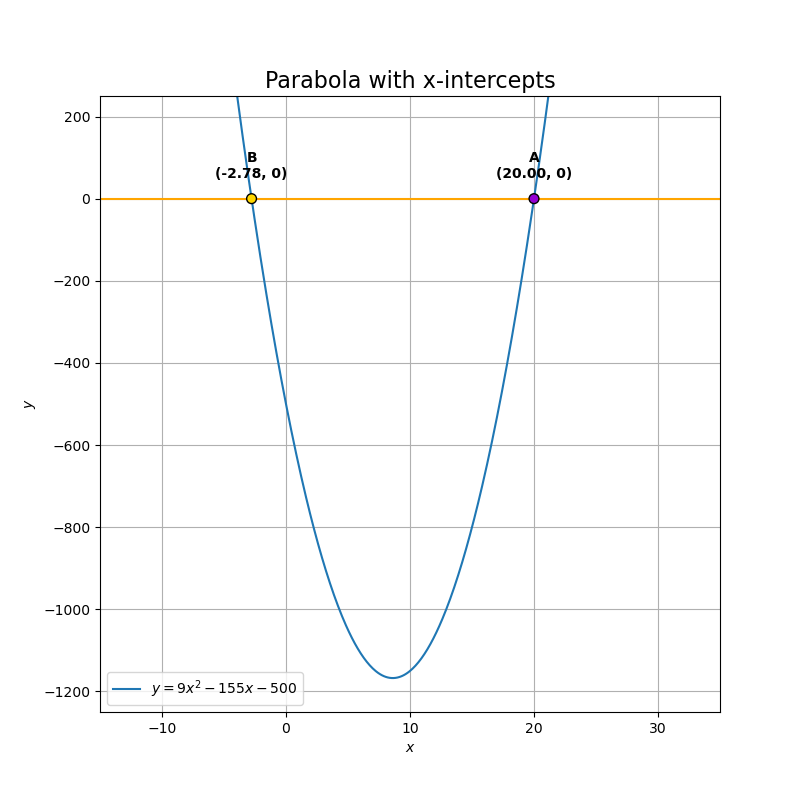
\includegraphics[width=0.7\columnwidth]{figs/Figure_1.png}
    \label{fig:placeholder}
    \caption{1}
\end{figure}
\end{frame}
\end{document}
